\chapter{Diseño de la metodología propuesta}

\section{Tecnologías de interfaz de usuario en el contexto bancario}

\subsection{Definición de tecnologías de interfaz de usuario}

Las tecnologías de interfaz de usuario comprenden el conjunto de herramientas,
frameworks, bibliotecas y metodologías que permiten desarrollar la interfaz de
usuario con la que interactúan los clientes y empleados de una institución
bancaria. Estos componentes tecnológicos constituyen la capa de presentación
que facilita la comunicación entre los usuarios y los sistemas bancarios
subyacentes.

En el contexto específico de las instituciones bancarias, las tecnologías
de interfaz de usuario deben satisfacer requisitos particularmente exigentes en términos de
seguridad, rendimiento, accesibilidad y cumplimiento normativo. Como define
Hassan (2022): ``Las tecnologías de interfaz de usuario en el sector bancario no solo
representan la interfaz visual, sino que constituyen un componente crítico del
sistema de seguridad y la estrategia de experiencia del cliente de la
institución''.

\subsection{Frameworks de interfaz de usuario}

Los frameworks de interfaz de usuario son estructuras predefinidas, conjuntos de
herramientas y bibliotecas que proporcionan funcionalidades reutilizables
para el desarrollo de interfaces de usuario. En el contexto bancario, estos
marcos deben satisfacer requisitos específicos:

\begin{enumerate}
  \item \textbf{React:} biblioteca desarrollada por Facebook que implementa un
        paradigma de componentes reutilizables y un flujo de datos
        unidireccional. Su flexibilidad arquitectónica permite construir
        interfaces complejas manteniendo un alto rendimiento.
  \item \textbf{Angular:} framework completo mantenido por Google que
        implementa el patrón MVVM (Modelo-Vista-VistaModelo). Proporciona
        funcionalidades robustas para aplicaciones empresariales como
        inyección de dependencias, sistema de tipos fuerte (TypeScript) y
        herramientas integradas para testing.
  \item \textbf{Vue.js:} framework progresivo que permite adopción incremental.
        Combina aspectos de React y Angular, ofreciendo un equilibrio entre
        funcionalidad y simplicidad.
  \item \textbf{Micro-frontends:} arquitectura que descompone interfaces
        monolíticas en aplicaciones más pequeñas, permitiendo a equipos
        independientes desarrollar, probar y desplegar componentes de forma
        autónoma.
\end{enumerate}

Como señala Zhang (2023): ``La selección del framework adecuado en el sector
bancario no solo determina la experiencia del usuario final, sino que impacta
directamente en la capacidad de la institución para responder ágilmente a
cambios regulatorios y expectativas del mercado''.

\subsection{Tecnologías complementarias}

Además de los frameworks principales, las soluciones de interfaz de usuario bancarias
incorporan diversas tecnologías complementarias:

\begin{enumerate}
  \item \textbf{Gestores de estado:} Redux, MobX, NgRx, Vuex --- fundamentales
        para gestionar datos complejos y flujos transaccionales.
  \item \textbf{Bibliotecas de componentes UI:} Material UI, Ant Design,
        Bootstrap --- aceleran el desarrollo y garantizan consistencia visual.
  \item \textbf{Herramientas de testing:} Jest, Cypress, Selenium ---
        esenciales para verificar funcionalidad y seguridad.
  \item \textbf{Herramientas de optimización:} Webpack, Rollup, Vite ---
        críticas para garantizar rendimiento óptimo.
  \item \textbf{Tecnologías de accesibilidad:} ARIA, herramientas de auditoría
        de accesibilidad --- necesarias para cumplimiento normativo e
        inclusión.
\end{enumerate}

\section{Instituciones bancarias y su contexto tecnológico}

\subsection{Características distintivas del sector bancario}

Las instituciones bancarias operan en un contexto único caracterizado por:

\begin{enumerate}
  \item \textbf{Alta regulación:} deben cumplir con numerosas normativas
        nacionales e internacionales que evolucionan constantemente.
  \item \textbf{Requisitos de seguridad elevados:} protección contra fraude,
        ciberataques y vulnerabilidades que podrían comprometer activos
        financieros.
  \item \textbf{Necesidad de estabilidad:} los sistemas bancarios requieren
        alta disponibilidad y tolerancia a fallos.
  \item \textbf{Integración de sistemas legacy:} frecuentemente deben
        interoperar con sistemas mainframe y arquitecturas heredadas.
  \item \textbf{Evolución digital acelerada:} presión para innovar frente a
        competidores digitales y fintech.
\end{enumerate}

Como sintetiza el estudio de Deloitte (2023): ``Las instituciones bancarias
enfrentan el desafío único de mantener la confianza y estabilidad esperadas
por sus clientes mientras aceleran su transformación digital para competir en
un ecosistema financiero radicalmente transformado''.

\subsection{Arquitectura tecnológica bancaria}

La arquitectura tecnológica típica de una institución bancaria presenta
múltiples capas:

\begin{enumerate}
  \item \textbf{Sistemas core bancarios:} generalmente sistemas legacy que
        gestionan las operaciones fundamentales (cuentas, préstamos, etc.).
  \item \textbf{Middleware y servicios de integración:} facilitan la
        comunicación entre sistemas core y aplicaciones modernas.
  \item \textbf{APIs y servicios:} exponen funcionalidades bancarias para su
        consumo por aplicaciones internas y externas.
  \item \textbf{Capa de presentación (de interfaz de usuario):} interfaces web, móviles y
        otros canales de interacción con clientes y empleados.
  \item \textbf{Infraestructura de seguridad:} sistemas transversales que
        garantizan autenticación, autorización y protección de datos.
\end{enumerate}

Las tecnologías de interfaz de usuario deben integrarse armoniosamente en esta
arquitectura compleja, respetando sus restricciones y aprovechando sus
capacidades.

\subsection{Tendencias de transformación digital bancaria}

El sector bancario está experimentando transformaciones significativas que
impactan directamente en los requisitos para tecnologías de interfaz de usuario:

\begin{enumerate}
  \item \textbf{Omnicanalidad:} experiencia consistente e integrada a través
        de múltiples canales (web, móvil, cajeros, sucursales).
  \item \textbf{Personalización basada en datos:} interfaces adaptativas que
        responden al comportamiento y preferencias individuales.
  \item \textbf{Open Banking:} exposición de servicios bancarios a través de
        APIs para integración con terceros.
  \item \textbf{Inteligencia artificial y automatización:} incorporación de
        asistentes virtuales y sistemas predictivos en interfaces.
  \item \textbf{Biometría y autenticación avanzada:} métodos de verificación
        de identidad más seguros y convenientes.
\end{enumerate}

\section{Criterios de evaluación y selección tecnológica}

\subsection{Criterios técnicos}

La evaluación técnica de tecnologías de interfaz de usuario para el sector
bancario contempla seis criterios, ponderados en la Tabla \ref{tab:3.1}:

\begin{enumerate}
  \item \textbf{Seguridad:}
  \begin{itemize}
    \item Protección contra vulnerabilidades comunes (XSS, CSRF)
    \item Soporte para políticas de seguridad de contenido (CSP)
    \item Capacidades de sanitización de datos
    \item Actualización y gestión de dependencias
  \end{itemize}
  \item \textbf{Rendimiento y escalabilidad:}
  \begin{itemize}
    \item Tiempo de carga inicial (First Contentful Paint) y tiempo hasta
          interactividad (Time to Interactive)
    \item Rendimiento en dispositivos de gama baja y redes móviles variables
    \item Rendimiento con grandes volúmenes de datos y estados complejos
    \item Soporte para múltiples equipos de desarrollo y división modular
          (\emph{code splitting})
  \end{itemize}
  \item \textbf{Mantenibilidad:}
  \begin{itemize}
    \item Estructura del código y modularidad
    \item Facilidad para testing automatizado
    \item Claridad y consistencia arquitectónica
    \item Documentación y soporte comunitario
  \end{itemize}
  \item \textbf{Calidad y verificabilidad del código generado por IA} (criterio
        emergente):
  \begin{itemize}
    \item Consistencia arquitectónica de las sugerencias de asistentes de
          código (Copilot, Cursor) frente al patrón oficial del framework
    \item Facilidad de revisión y auditoría del código generado por IA
    \item Disponibilidad de reglas de \emph{linting} y tipado que acoten el
          espacio de sugerencias válidas
    \item Trazabilidad entre el código generado y el prompt/contexto que lo
          originó
  \end{itemize}
  \item \textbf{Accesibilidad:}
  \begin{itemize}
    \item Conformidad con estándares WCAG 2.1
    \item Soporte para tecnologías asistivas
    \item Herramientas integradas para validación de accesibilidad
    \item Navegación por teclado y compatibilidad con lectores de pantalla
  \end{itemize}
  \item \textbf{Compatibilidad multiplataforma:}
  \begin{itemize}
    \item Soporte consistente entre navegadores (\emph{cross-browser})
    \item Adaptabilidad a múltiples dispositivos y tamaños de pantalla
    \item Consistencia de experiencia entre canales web, móvil y cajeros
          (omnicanalidad bancaria)
    \item Compatibilidad con versiones anteriores de navegadores corporativos
  \end{itemize}
\end{enumerate}

\subsection{Factores organizacionales: por qué se excluyen del modelo ponderado}

Las metodologías genéricas de evaluación tecnológica —incluida una versión
previa de este modelo— suelen incorporar factores organizacionales como
criterios de ponderación independientes:

\begin{itemize}
  \item \textbf{Ecosistema y comunidad:} tamaño y actividad de la comunidad
        de desarrolladores, disponibilidad de recursos y formación,
        continuidad y roadmap del proyecto.
  \item \textbf{Talento y curva de aprendizaje:} disponibilidad de
        desarrolladores en el mercado, facilidad de adopción por equipos
        existentes, transferencia de conocimiento intraorganizacional.
  \item \textbf{Alineación estratégica:} compatibilidad con la visión
        tecnológica de la organización y su roadmap de mediano plazo.
\end{itemize}

La presente metodología excluye deliberadamente estos factores como
criterios de ponderación independientes, no porque hayan dejado de existir,
sino porque la evidencia reciente sobre productividad de desarrolladores
asistidos por Inteligencia Artificial (Peng et al., 2023; Stack Overflow, 2024)
muestra que la brecha de talento y curva de aprendizaje entre frameworks se
reduce significativamente cuando el equipo utiliza asistentes de código
generativo: un desarrollador con experiencia media, apoyado por IA, alcanza
niveles de productividad comparables en un framework que no domina en un
plazo sustancialmente menor al histórico. Mantener estos factores como ejes
de ponderación independientes introduciría en el modelo una fuente de
varianza que la práctica actual del desarrollo de software ya no sostiene con
la misma fuerza que hace pocos años, y que resulta además ajena tanto a las
propiedades técnicas del framework como a las exigencias regulatorias del
sector --los dos ejes que dan nombre a esta investigación. El efecto de esta
exclusión se cuantifica empíricamente en el Capítulo 4 (sección 4.2.4,
escenario S3), donde se compara la decisión resultante con y sin los
criterios asociados a la IA generativa.

El costo total de propiedad (licencias, formación, migración y mantenimiento)
se conserva como información contextual para la Fase 3 del proceso
decisional (sección 3.4), pero tampoco integra la matriz de ponderación por
tratarse de un factor económico-organizacional, no técnico ni regulatorio.

\subsection{Criterios específicos del sector bancario}

Las instituciones bancarias deben considerar criterios particulares derivados
de su contexto operativo:

\begin{enumerate}
  \item \textbf{Cumplimiento regulatorio:}
  \begin{itemize}
    \item Capacidad para implementar requisitos de accesibilidad legal
    \item Soporte para auditoría y trazabilidad de acciones
    \item Adaptabilidad ante cambios normativos
    \item Conformidad con estándares específicos del sector (PCI-DSS, etc.)
  \end{itemize}
  \item \textbf{Integración con sistemas legacy:}
  \begin{itemize}
    \item Compatibilidad con arquitecturas existentes
    \item Capacidad de comunicación con sistemas mainframe
    \item Estrategias de adaptación y \emph{wrapping}
    \item Coexistencia durante transiciones graduales
  \end{itemize}
  \item \textbf{Requisitos de alta disponibilidad:}
  \begin{itemize}
    \item Tolerancia a fallos y degradación elegante
    \item Estrategias de caché y funcionamiento offline
    \item Recuperación ante errores de red o backend
    \item Garantías de SLA (Acuerdos de Nivel de Servicio)
  \end{itemize}
  \item \textbf{Gobernanza regulatoria del uso de IA generativa en desarrollo}
        (criterio emergente):
  \begin{itemize}
    \item Trazabilidad y procedencia (\emph{provenance}) del código sugerido
          por herramientas de IA, exigible en auditorías SBS/PCI-DSS
    \item Gestión del riesgo de propiedad intelectual y licenciamiento del
          código generado por modelos de lenguaje entrenados con datos
          externos
    \item Políticas de gobernanza de datos para el uso de asistentes de IA
          sobre código fuente bancario sensible
    \item Disponibilidad de mecanismos de revisión humana obligatoria
          (\emph{human-in-the-loop}) antes del despliegue a producción
  \end{itemize}
\end{enumerate}

\subsection{Matriz de ponderación de criterios de evaluación}

La importancia relativa de cada criterio varía según el contexto institucional
específico. Para la presente metodología, la ponderación fue derivada mediante
consenso de expertos aplicando la Técnica Delphi con doce especialistas del
sector bancario (líderes técnicos, arquitectos empresariales y oficiales de
cumplimiento), en una segunda ronda que incorporó explícitamente los dos
criterios emergentes asociados a la IA generativa. La Tabla \ref{tab:3.1}
presenta los pesos resultantes, organizados en las dos dimensiones que dan
nombre a la metodología: técnica y regulatoria.

El modelo consolida diez criterios de evaluación: seis técnicos, que en
conjunto concentran el 60\% del peso total, y cuatro regulatorios/bancarios,
que concentran el 40\% restante. Los criterios organizacionales
tradicionales (ecosistema, talento, alineación estratégica) fueron
retirados de la ponderación por las razones expuestas en la sección
anterior; su peso combinado en el modelo previo (20\%) fue redistribuido
hacia los ocho criterios técnico-regulatorios preexistentes y hacia los dos
criterios emergentes de IA (calidad del código generado por IA: 0.08;
gobernanza regulatoria de IA: 0.06), que en conjunto reciben el 14\% del
peso total --una magnitud deliberadamente menor a la de los criterios de
seguridad y cumplimiento, pero suficiente para reflejar su relevancia
creciente sin subordinar los fundamentos técnicos y regulatorios clásicos
del modelo.

La Figura \ref{fig:3.1} visualiza la magnitud relativa de cada uno de los
diez pesos, y la Figura \ref{fig:3.2} desglosa la composición del modelo en
sus dos dimensiones.

\begin{figure}[htbp]
\centering
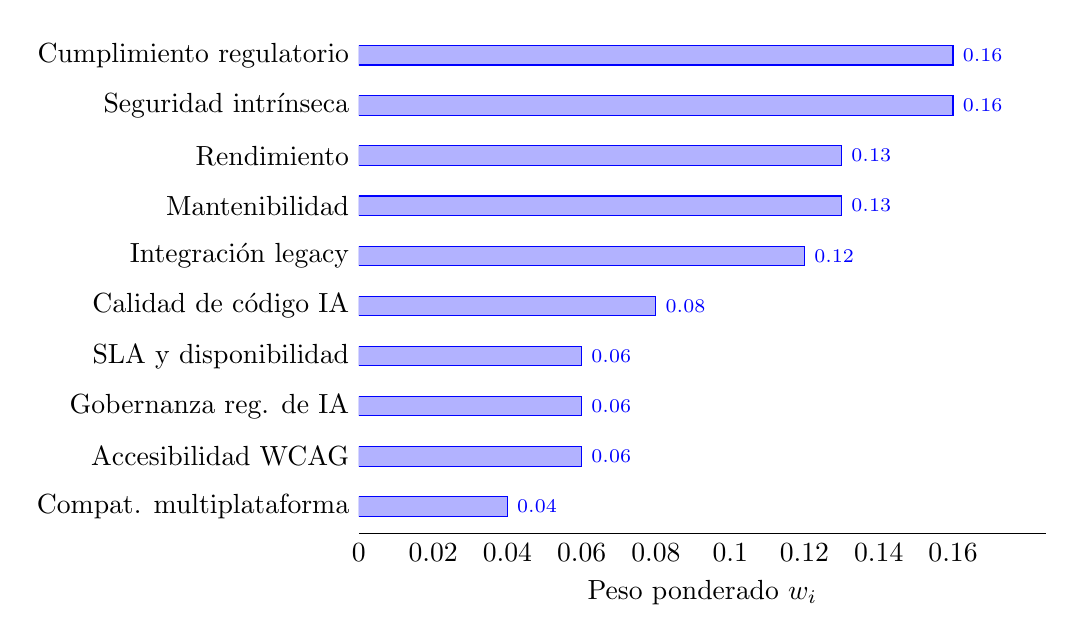
\begin{tikzpicture}
\begin{axis}[
  xbar,
  y axis line style = {opacity=0},
  axis x line = bottom,
  axis line style = {-},
  tickwidth = 0pt,
  enlarge y limits = 0.06,
  xmin = 0, xmax = 0.185,
  xtick = {0,0.02,0.04,0.06,0.08,0.10,0.12,0.14,0.16},
  scaled x ticks = false,
  /pgf/number format/.cd, fixed, precision=2,
  xlabel = {Peso ponderado $w_i$},
  symbolic y coords = {
    Compat. multiplataforma, Accesibilidad WCAG, Gobernanza reg. de IA,
    SLA y disponibilidad, Calidad de código IA, Integración legacy,
    Mantenibilidad, Rendimiento, Seguridad intrínseca,
    Cumplimiento regulatorio
  },
  ytick = data,
  width = 0.85\textwidth,
  height = 8cm,
  nodes near coords,
  nodes near coords align = horizontal,
  every node near coord/.append style = {font=\scriptsize},
  bar width = 7pt,
]
\addplot coordinates {
  (0.04,Compat. multiplataforma)
  (0.06,Accesibilidad WCAG)
  (0.06,Gobernanza reg. de IA)
  (0.06,SLA y disponibilidad)
  (0.08,Calidad de código IA)
  (0.12,Integración legacy)
  (0.13,Mantenibilidad)
  (0.13,Rendimiento)
  (0.16,Seguridad intrínseca)
  (0.16,Cumplimiento regulatorio)
};
\end{axis}
\end{tikzpicture}
\caption{Pesos ponderados $w_i$ de los diez criterios de evaluación obtenidos mediante AHP. Los dos criterios asociados a la IA generativa se señalan con su dimensión (téc./reg.)}
\label{fig:3.1}
\end{figure}

\begin{figure}[htbp]
\centering
\begin{tikzpicture}
\pie[
  radius=3,
  color={gray!70,gray!30},
  text=legend
]{60/Criterios técnicos (60\%), 40/Criterios regulatorios (40\%)}
\end{tikzpicture}
\caption{Distribución de los diez criterios en las dos dimensiones del modelo: técnica y regulatoria}
\label{fig:3.2}
\end{figure}

\begin{table}[htbp]
\centering
\caption{Matriz de ponderación de criterios de evaluación para el sector bancario}
\label{tab:3.1}
\small
\begin{tabular}{@{}p{4.6cm}p{2cm}p{1.3cm}p{5cm}@{}}
\toprule
Criterio & Dimensión & Peso ($w_i$) & Justificación \\
\midrule
Seguridad y protección              & Técnica     & 0.16 & Requisito crítico e indelegable en banca \\
Rendimiento y escalabilidad         & Técnica     & 0.13 & Picos de tráfico hasta 20$\times$ la base \\
Mantenibilidad del código           & Técnica     & 0.13 & Equipos grandes, proyectos plurianuales \\
Calidad del código generado por IA  & Técnica     & 0.08 & Consistencia y auditabilidad del código asistido por IA (criterio emergente) \\
Accesibilidad (WCAG 2.2)            & Técnica     & 0.06 & Obligación normativa e inclusión financiera \\
Compatibilidad multiplataforma      & Técnica     & 0.04 & Omnicanalidad bancaria \\
Cumplimiento regulatorio            & Regulatoria & 0.16 & PCI-DSS, DORA, normativas SBS/locales \\
Integración con sistemas legacy     & Regulatoria & 0.12 & Arquitecturas heterogéneas (15+ años) \\
Alta disponibilidad (SLA)           & Regulatoria & 0.06 & Criticidad operacional -- US\$67k/min caída \\
Gobernanza regulatoria del uso de IA & Regulatoria & 0.06 & Trazabilidad y riesgo de IP del código IA-asistido (criterio emergente) \\
\midrule
\textbf{Total} & & \textbf{1.00} & \\
\bottomrule
\end{tabular}
\end{table}

\section{Proceso estructurado de toma de decisiones}

La metodología integral propuesta para la selección de tecnologías de interfaz de usuario
en instituciones bancarias se estructura en cuatro fases secuenciales e
integradas. Cada fase produce entregables concretos que alimentan la fase
siguiente, garantizando la trazabilidad del proceso decisional y la coherencia
entre las dos dimensiones del modelo: técnica y regulatoria. Esta
estructura supera las limitaciones de los enfoques genéricos de evaluación
tecnológica identificadas en la revisión de la literatura (Jansen y Lee, 2011).

La Tabla \ref{tab:3.2} presenta la descripción sintética de cada fase, sus
actividades principales y los entregables esperados. La Fase 3, antes
denominada ``Valoración Estratégica'' en versiones previas de este modelo, se
redefine como \textbf{Evaluación Regulatoria y de Gobernanza de IA},
consistente con la exclusión de los factores organizacionales discutida en
la sección 3.3.2: su contenido deja de girar en torno al talento y al
roadmap estratégico, y pasa a profundizar el cumplimiento normativo y la
gobernanza del uso de IA generativa que la Fase 2 identifica a nivel técnico.

La secuencialidad de las fases no implica rigidez lineal: se contemplan
mecanismos de retroalimentación entre fases adyacentes. Si durante la Fase 2
(Evaluación Técnica) se identifican restricciones regulatorias no
documentadas en la Fase 1, el proceso retrocede formalmente a completar el
análisis de requisitos antes de continuar. Asimismo, si el consenso no se
alcanza en la Fase 4, el comité evaluador puede solicitar una revisión de la
Fase 3.

\begin{table}[htbp]
\centering
\caption{Fases de la metodología propuesta para la selección de tecnologías de interfaz de usuario (modelo técnico-regulatorio)}
\label{tab:3.2}
\small
\begin{tabular}{@{}p{0.5cm}p{2.7cm}p{5.2cm}p{4.3cm}@{}}
\toprule
N.\textsuperscript{o} & Fase & Actividades principales & Entregables \\
\midrule
1 & Análisis de Requisitos Institucionales
  & Relevamiento de requisitos técnicos y regulatorios; mapeo de arquitectura existente; identificación de restricciones normativas
  & Documento de requisitos; inventario de restricciones; perfil institucional \\
\addlinespace
2 & Evaluación Técnica Específica
  & Benchmarking técnico de Angular, React y Vue.js; aplicación de la matriz AHP; evaluación de la calidad del código generado por IA
  & Scorecard técnico comparativo; informe de calidad de código IA-asistido \\
\addlinespace
3 & Evaluación Regulatoria y de Gobernanza de IA
  & Verificación de cumplimiento normativo (PCI-DSS, DORA, SBS); evaluación de gobernanza y riesgo del uso de IA generativa; análisis del costo total de propiedad (TCO) a 5 años
  & Informe de brechas regulatorias; matriz de gobernanza de IA; análisis TCO comparado \\
\addlinespace
4 & Decisión Final Estructurada
  & Consolidación de evaluaciones técnicas y regulatorias; deliberación del comité de stakeholders; validación por el Arquitecto Principal
  & Acta de decisión; justificación documentada; plan de adopción \\
\bottomrule
\end{tabular}
\end{table}

\subsection{Implementación y roles del proceso decisional}

La ejecución efectiva de la metodología requiere la participación coordinada
de múltiples roles institucionales siguiendo una matriz RACI (\emph{Responsible,
Accountable, Consulted, Informed}). El proceso es liderado por el Arquitecto
Empresarial Principal (\emph{Accountable}), con participación activa del equipo de
seguridad (CISO), los líderes técnicos de desarrollo, los oficiales de
cumplimiento regulatorio y un responsable de gobernanza de datos e IA
--rol que audita específicamente el criterio de gobernanza regulatoria de
IA generativa (sección 3.3.3)--; a diferencia de versiones previas del
modelo, no se requiere un rol dedicado a la validación estratégica de
negocio, dado que el modelo técnico-regulatorio no pondera ese eje. Esta estructura evita los
patrones de fragmentación decisional documentados en el diagnóstico:
decisiones técnicas sin verificación regulatoria, o decisiones regulatorias
sin respaldo técnico suficiente (L. Chen et al., 2021).

El tiempo estimado de ejecución completa para una institución bancaria de
tamaño mediano es de seis a ocho semanas, distribuidas aproximadamente de la
siguiente manera: Fase 1 (dos semanas), Fase 2 (dos semanas), Fase 3 (una
semana) y Fase 4 (una a tres semanas, según la complejidad del proceso de
consenso regulatorio). Las instituciones con mayor madurez en gobernanza
tecnológica pueden completar el proceso en el extremo inferior de este rango.
